\section{The obstruction on ten labels}\label{sec:ten-labels}

We prove that an admissible map $\mathbb{RP}^3\to\Delta^9$ cannot exist.
Its support complex would have tetrahedral facets. Each facet forces a
six-label triangle system on its complement; transporting these systems
between adjacent facets will constrain the whole complex.

\begin{lemma}\label{lem:facet-complement}
Suppose $f:\mathbb{RP}^3\to\Delta^9$ is admissible, let $K$ be its support
complex, and let $S$ be a tetrahedron of $K$. The triangles of $K$
contained in the six-element set $C=[10]\setminus S$ form a six-label
triangle system. In particular, two tetrahedra of $K$ cannot be disjoint.
\end{lemma}

\begin{proof}
Theorem~\ref{thm:equality-complex} says that $K$ is pure of
dimension three. A witness line $x$ for the facet $S$ has support exactly
$S$. The restriction of $f$ to $\mathbb P(x^\perp)\cong\mathbb{RP}^2$
uses only labels in $C$. It uses all six: otherwise the lower bound in
Proposition~\ref{thm:label-bound}, applied in dimension three,
would be violated. By Lemma~\ref{lem:six-from-map}, this restriction
supplies a six-label triangle system contained among the triangles of
$K$ on $C$.

There are no additional triangles on $C$. Otherwise some complementary
triples $T,C\setminus T$ would both be triangles of $K$. Take witness
lines for $S,T,C\setminus T$. In $\mathbb R^4$ there is a line
perpendicular to all three; their supports together contain all ten
labels, leaving that line no admissible label.

If a tetrahedron $S'$ were disjoint from $S$, its four triples would all
be triangles on $C$. This contradicts
Lemma~\ref{lem:six-properties}(2).
\end{proof}

The rest of the proof is purely combinatorial. We retain the notation
$K$ and write $\mathcal T_C$ for the triangle system on a facet
complement $C$. By Theorem~\ref{thm:equality-complex}, each
triangle of $K$ lies in a positive even number of tetrahedra.

\begin{lemma}\label{lem:two-tetrahedra}
Every triangle of $K$ belongs to exactly two tetrahedra.
\end{lemma}

\begin{proof}
First observe that if two tetrahedra differ by exchanging labels $a,b$,
the same exchange carries their complementary triangle systems to one
another. Their complements share five labels, on which both systems are
the triangles of $K$. After the exchange these triangles remain fixed,
so the systems agree everywhere by
Lemma~\ref{lem:six-properties}(4).

Suppose three tetrahedra $T\cup\{a\}$, $T\cup\{b\}$,
$T\cup\{c\}$ contain the same triangle $T$. Put
$R=[10]\setminus(T\cup\{a,b,c\})$, which has four elements. Transporting
the complementary systems successively by
\[
 R\cup\{b,c\}
 \xrightarrow{(a\ b)}R\cup\{a,c\}
 \xrightarrow{(b\ c)}R\cup\{a,b\}
 \xrightarrow{(c\ a)}R\cup\{b,c\}
\]
preserves the initial system. The composite fixes $R$ and exchanges $b$
and $c$, contradicting Lemma~\ref{lem:six-properties}(3). Thus at most
two tetrahedra contain any triangle. Positive even multiplicity gives
exactly two.
\end{proof}

For an edge $D$ of $K$, define its \emph{link graph} to have as vertices
the labels $v\notin D$ for which $D\cup\{v\}$ is a triangle, and as
edges the pairs $\{v,w\}$ for which $D\cup\{v,w\}$ is a tetrahedron.

\begin{lemma}\label{lem:short-links}
Every connected component of an edge link is a cycle of length three
or four.
\end{lemma}

\begin{proof}
Every vertex of an edge link has degree two by
Lemma~\ref{lem:two-tetrahedra}, so each component is a simple cycle.
We show that the link contains no path on five distinct vertices.

Suppose such a path has consecutive vertices $v_0,v_1,v_2,v_3,v_4$.
Let $R$ be the three labels outside $D\cup\{v_0,v_1,v_2,v_3,v_4\}$.
The four successive edges give tetrahedra
$D\cup\{v_i,v_{i+1}\}$, whose complementary systems are transported by
\[
\begin{aligned}
 R\cup\{v_2,v_3,v_4\}
 &\xrightarrow{(v_0\ v_2)} R\cup\{v_0,v_3,v_4\}
 \xrightarrow{(v_1\ v_3)} R\cup\{v_0,v_1,v_4\}\\
 &\xrightarrow{(v_2\ v_4)} R\cup\{v_0,v_1,v_2\}.
\end{aligned}
\]
The composite fixes $R$ and sends $v_4$ to $v_2$. Hence for every pair
$\{r,s\}\subset R$, the first system contains $\{v_4,r,s\}$ if and
only if the last contains $\{v_2,r,s\}$. The latter triple belongs to
both complementary sets, so its membership in either system is simply
its membership in $K$. The first system therefore has identical link
graphs at $v_4$ and $v_2$ when restricted to $R$. This contradicts
Lemma~\ref{lem:six-properties}(3). Every cycle of length at least five
contains such a path, proving the assertion.
\end{proof}

The short links let us describe every facet obtained by repeatedly
crossing a triangular face of one fixed tetrahedron. The description
will produce enough facets to contradict the complementary triangle
system.

\begin{lemma}\label{lem:partner-blocks}
Fix a tetrahedron $S$ of $K$. For $v\in S$, let $p(v)$ be the unique
label outside $S$ such that
$(S\setminus\{v\})\cup\{p(v)\}$ is a tetrahedron. For each distinct
value $y$ of $p$, set
\[
 B_y=p^{-1}(y)\cup\{y\}.
\]
The sets $B_y$ are disjoint and have at least two elements. For every
choice $q_y\in B_y$, the set
\[
 \bigcup_{y\in p(S)}(B_y\setminus\{q_y\})
\]
is a tetrahedron. Moreover, every tetrahedron of $K$ contains at least two
elements of one of these blocks.
\end{lemma}

\begin{proof}
The partner $p(v)$ exists and is unique by
Lemma~\ref{lem:two-tetrahedra}, applied to $S\setminus\{v\}$. It lies
outside $S$, since the only tetrahedron on the vertices of $S$ is $S$
itself. The stated disjointness and lower size bound are immediate.

We first prove that replacing $v$ by $a=p(v)$ leaves the collection of
blocks unchanged. Put $S'=(S\setminus\{v\})\cup\{a\}$ and let $p'$
be its partner map. We have $p'(a)=v$. For $w\in S\setminus\{v\}$,
put $D=S\setminus\{v,w\}$ and $b=p(w)$. The link of $D$ contains
the edges
\[
 \{v,w\},\qquad \{w,a\},\qquad \{v,b\}.
\]
If $a=b$, these form a three-cycle. Since every link vertex has degree
two, that cycle is a whole component, and the other tetrahedron on
$D\cup\{a\}$ is $D\cup\{a,v\}$. Thus $p'(w)=v$.
If $a\ne b$, the displayed edges form the path $a,w,v,b$ on four
distinct vertices. Lemma~\ref{lem:short-links} forces it to complete
to a four-cycle, with the edge $\{a,b\}$. Thus $p'(w)=b=p(w)$.
The two cases are illustrated in Figure~\ref{fig:partner-links}.
We have proved
\[
 p'(a)=v,\qquad
 p'(w)=
 \begin{cases}
 v,&p(w)=a,\\
 p(w),&p(w)\ne a.
 \end{cases}
\]
\begin{figure}[tbp]
\centering
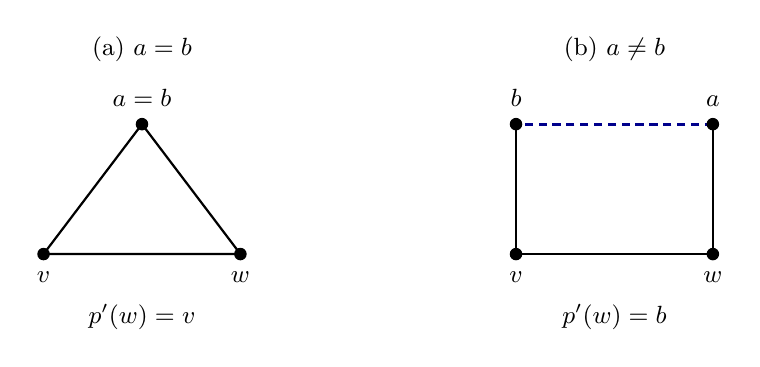
\begin{tikzpicture}[
  x=1cm,y=1cm,font=\small,
  vertex/.style={circle,fill=black,inner sep=1.6pt},
  every path/.style={line width=.8pt}
]
\node at (1.25,2.6) {(a) $a=b$};
\node at (7.25,2.6) {(b) $a\ne b$};
\draw (0,0)--(2.5,0)--(1.25,1.65)--cycle;
\node[vertex,label=below:$v$] at (0,0) {};
\node[vertex,label=below:$w$] at (2.5,0) {};
\node[vertex,label=above:{$a=b$}] at (1.25,1.65) {};
\node at (1.25,-.8) {$p'(w)=v$};
\draw (6,1.65)--(6,0)--(8.5,0)--(8.5,1.65);
\draw[blue!55!black,densely dashed,line width=1pt] (8.5,1.65)--(6,1.65);
\node[vertex,label=below:$v$] at (6,0) {};
\node[vertex,label=below:$w$] at (8.5,0) {};
\node[vertex,label=above:$b$] at (6,1.65) {};
\node[vertex,label=above:$a$] at (8.5,1.65) {};
\node at (7.25,-.8) {$p'(w)=b$};
\end{tikzpicture}
\caption{The two partner updates in the link of
$D=S\setminus\{v,w\}$. Put $a=p(v)$ and $b=p(w)$, and replace
$v$ by $a$ in the tetrahedron $S$. The new partner map is $p'$.
The known edges $\{v,w\}$, $\{w,a\}$ and $\{v,b\}$ form a triangle
when $a=b$. When $a\ne b$, they form a path on four vertices; the
short-link condition forces the closing edge $\{a,b\}$ (dashed).
In both cases $p'(a)=v$, and the blocks retain their elements.}
\label{fig:partner-links}
\end{figure}


The block formerly indexed by $a$ is now indexed by $v$ and has the
same elements; all other blocks are unchanged.

The tetrahedron $S$ contains all elements of each block except its
indexing partner. The same is true after any such exchange, by block
invariance. To change the omitted element of a block from $q$ to $u$,
replace the present element $u$ by its partner $q$. Doing this once
in each block where a change is wanted realizes every possible choice
of omissions. These sets have cardinality four, since
$\sum_y(|B_y|-1)=|S|=4$.

Finally, suppose a tetrahedron $T$ met each block in at most one
element. In each block omit that element if present, and otherwise
omit any element. The resulting tetrahedron lies in the union of the
blocks and is disjoint from $T$, contrary to
Lemma~\ref{lem:facet-complement}.
\end{proof}

\begin{theorem}\label{thm:no-ten-labels}
There is no admissible map $\mathbb{RP}^3\to\Delta^9$.
\end{theorem}

\begin{proof}
Assume such a map exists and fix a tetrahedron $S$ of its support
complex. Let $t$ be the number of blocks in
Lemma~\ref{lem:partner-blocks}, and let $R$ be the set of labels outside
their union. The blocks contain $4+t$ labels in total, so
\[
 1\le t\le4,\qquad |R|=6-t.
\]
If $t=4$, each block has size two and $S$ meets each in just one
element, contradicting the last assertion of
Lemma~\ref{lem:partner-blocks}. Thus $t\le3$.

There is no triangle entirely in $R$. By purity, such a triangle would
extend to a tetrahedron; its one remaining vertex could not supply two
vertices in a block. On the other hand, $R$ is contained in
$[10]\setminus S$, where every four labels contain a triangle by
Lemmas~\ref{lem:facet-complement} and~\ref{lem:six-properties}(2).
Consequently $|R|\le3$, and therefore $t\ge3$.

It follows that $t=3$, $|R|=3$, and the block sizes are $3,2,2$,
as in Figure~\ref{fig:partner-blocks}.
\begin{figure}[tbp]
\centering
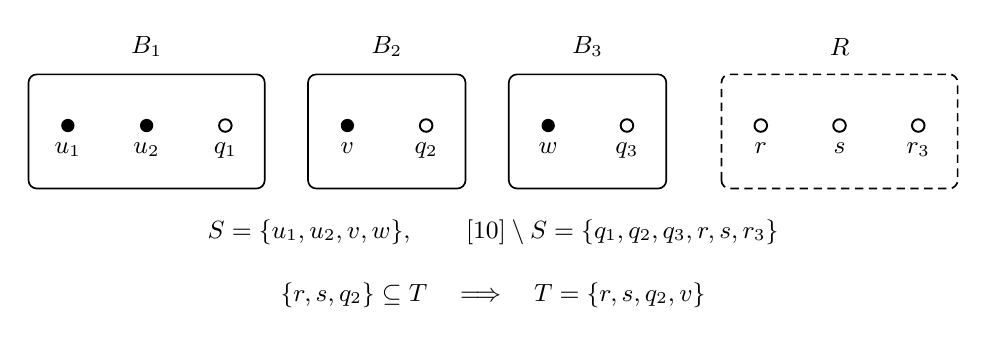
\begin{tikzpicture}[
  x=1cm,y=1cm,font=\small,
  present/.style={circle,fill=black,inner sep=1.7pt},
  omitted/.style={circle,draw=black,fill=white,inner sep=1.6pt,line width=.7pt},
  every path/.style={line width=.6pt}
]
\draw[rounded corners=3pt] (0,.35) rectangle (3,1.8);
\draw[rounded corners=3pt] (3.55,.35) rectangle (5.55,1.8);
\draw[rounded corners=3pt] (6.1,.35) rectangle (8.1,1.8);
\draw[rounded corners=3pt,densely dashed] (8.8,.35) rectangle (11.8,1.8);
\node at (1.5,2.15) {$B_1$};
\node at (4.55,2.15) {$B_2$};
\node at (7.1,2.15) {$B_3$};
\node at (10.3,2.15) {$R$};
\node[present,label=below:$u_1$] at (.5,1.15) {};
\node[present,label=below:$u_2$] at (1.5,1.15) {};
\node[omitted,label=below:$q_1$] at (2.5,1.15) {};
\node[present,label=below:$v$] at (4.05,1.15) {};
\node[omitted,label=below:$q_2$] at (5.05,1.15) {};
\node[present,label=below:$w$] at (6.6,1.15) {};
\node[omitted,label=below:$q_3$] at (7.6,1.15) {};
\node[omitted,label=below:$r$] at (9.3,1.15) {};
\node[omitted,label=below:$s$] at (10.3,1.15) {};
\node[omitted,label=below:$r_3$] at (11.3,1.15) {};
\node at (5.9,-.2) {$S=\{u_1,u_2,v,w\},\qquad [10]\setminus S=\{q_1,q_2,q_3,r,s,r_3\}$};
\node at (5.9,-1) {$\{r,s,q_2\}\subseteq T\quad\Longrightarrow\quad T=\{r,s,q_2,v\}$};
\end{tikzpicture}
\caption{The only remaining block sizes are $3,2,2$, with three
labels in $R$ outside the blocks. Filled dots are the vertices of the
fixed tetrahedron $S$; the omitted block elements are $q_1,q_2,q_3$.
Every tetrahedron must contain two vertices of one block. After
relabeling the two-element blocks, the final argument selects a triangle
$\{r,s,q_2\}$ with $r,s\in R$. Its only possible tetrahedral extension
is obtained by adjoining $v$, contradicting the two required extensions.}
\label{fig:partner-blocks}
\end{figure}


The complement of $S$ consists of $R$ and one omitted element from
each block. Choose two distinct labels $r,s\in R$. In the triangle
system on this complement, $\{r,s\}$ belongs to two distinct triangles.
Their third vertices cannot be in $R$, because $R$ contains no
triangle. They are therefore two distinct omitted block elements.
Only one block has size three, so at least one of these triangles is
$\{r,s,z\}$ with $z$ in a block $B$ of size two.

Every tetrahedron containing $\{r,s,z\}$ must contain two vertices of
some block. As $r,s$ lie outside all blocks, its fourth vertex must be
the other element of $B$. Thus this triangle belongs to at most one
tetrahedron, contradicting Lemma~\ref{lem:two-tetrahedra}.
\end{proof}
